%%%%%%%%%%%%%%%%%%%%%%%%%%%%%%%%%%%%%%%%%%%%%%%%%%%%%%%%%%%%%%%%%%%%%%%%%%%%%%%%
\chapter{ПОСТАНОВКА ЗАДАЧИ, ВЫБОР СПОСОБА РЕШЕНИЯ}
%%%%%%%%%%%%%%%%%%%%%%%%%%%%%%%%%%%%%%%%%%%%%%%%%%%%%%%%%%%%%%%%%%%%%%%%%%%%%%%%
В современном мире коммуникации через интернет становятся очень удобными, и экономят время. Такие коммуникации особенно будут экономить время, если их встроить в CRM-системы. Поэтому задача будет написать модуль SIP-телефона для web-браузера, поддерживаемого как можно большим количеством браузеров, и легко в будущем встраиваемый в любое web-приложение, например, CRM-систему. В данной работе ограничимся только передачей аудио потока.

Для реализации данной задачи, будем использовать технологию WebRTC. Существуют две реализации технологии WebRTC по протоколу SIP на JavaScript: библиотека sipML5 и библиотека JsSIP.\cite{sipML5}\cite{JsSIP}

Размер библиотеки JsSIP ~130kb, но она требует установки Node.js на сервере. Размер библиотеки sipML5 чуть больше 1Mb.

Обе библиотеки довольно неплохие и имеют следующие преимущества:
\begin{enumerate}
\item хорошая документация
\item возможность осуществления аудио и видео звонков
\item возможность отправки мгновенных сообщений
\item поддержка статуса присутствия в сети
\item функция удержания вызова
\item функция отключения микрофона
\item тональный набор (DTMF)
\end{enumerate}

Помимо этого в библиотеке sipML5 имеется функции трансляции экрана (пока что только для Google Chrome), перенаправления вызова и группового звонка.

Хоть и обе библиотеки довольно хороши, для нашей задачи выберем библиотеку sipML5, потому что функциональность у неё больше и не нужно дополнительно устанавливать Node.js на сервер.

На рисунке \ref{image:modulesStructure} под номером 4 изображён разрабатываемый модуль.

\begin{figure}[h!]
\center{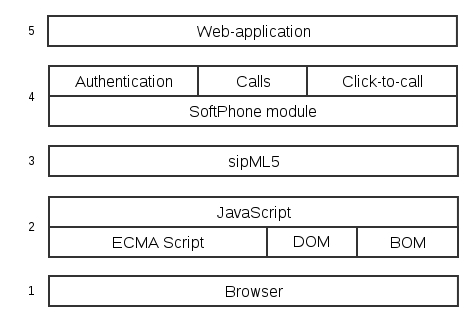
\includegraphics[width=0.5\linewidth]{modulesStructure}}
\caption{Структура взаимодействия модулей}
\label{image:modulesStructure}
\end{figure}